\documentclass[10pt,twocolumn]{article}
\usepackage[margin=0.72in,columnsep=0.22in]{geometry}
\usepackage{amsmath,booktabs,graphicx,microtype,xcolor,tikz,hyperref}
\usetikzlibrary{arrows.meta,positioning,fit,calc}
\hypersetup{colorlinks=true,linkcolor=blue!55!black,urlcolor=blue!60!black,citecolor=blue!55!black}
\title{Flash-flooplanner: A Metal-Aware and Process-Scalable Floorplanning Framework for Early-Stage IC Architecture Exploration}
\author{Liangdacheng \and GPT5.5-assisted development}
\date{Pixel Edition v8.6.1 -- Preprint}
\begin{document}
\maketitle
\begin{abstract}
Flash-flooplanner is an interactive early-stage IC floorplanning environment that connects architecture choices to process scaling, placement, metal-aware interconnect pressure, manufacturing yield, and cost. Version 8.6.1 adds first-class connection management with edge-anchored orthogonal buses, per-net horizontal/vertical metal-layer allocation, keyboard-oriented editing, and a CPU reference library spanning Arm Cortex, BOOM, XiangShan, NVIDIA Vera Olympus, and Tenstorrent Ocelot. The tool distinguishes measured, calibrated, estimated, and heuristic evidence. A held-out Nangate45/OpenROAD study reports 24.87\% area MAPE and demonstrates that an MST-plus-segment-union routing proxy raises mean Pearson congestion correlation from 0.430 to 0.737 relative to the original star adapter. These results validate a narrow proxy task rather than signoff accuracy across advanced nodes. The artifact is a client-side Pixel UI intended for rapid architecture exploration, not replacement of synthesis, STA, or detailed routing.
\end{abstract}
\section{Motivation}
Architecture decisions are often made before a complete RTL implementation, hard macros, timing constraints, or a stable package definition exist. At that stage, architects still need to answer questions that are fundamentally physical: whether the target die can contain the planned compute and memory blocks; whether PHY placement consumes critical edge length; whether a wide fabric produces local metal pressure; whether a hierarchical topology trades wirelength for switch area and latency; and whether a nominally denser process actually improves good-unit economics.

Conventional spreadsheets are fast but lose geometry and connectivity. Full place-and-route is physically grounded but requires implementation collateral that does not exist early enough. Flash-flooplanner targets the gap. Its design goal is not signoff prediction; it is a transparent, interactive model whose assumptions remain visible and calibratable.

Version 8.6.1 extends this goal in three ways. First, nets are persistent design objects rather than decorative lines. Second, wide buses are attached to explicit module edges and can consume multiple horizontal and vertical metal layers. Third, reusable CPU reference templates are separated into core logic, private cache, and shared-cache budgets so that process scaling does not silently double-count SRAM.

The user-facing interface adopts an industrial pixel style, but the underlying model is deliberately separated from presentation. The same project state can be exported as JSON, SVG, Draw.io, a poster, or a paper-oriented figure.

\section{Four-Layer Modeling Framework}
Figure~\ref{fig:framework} summarizes the methodology. Inputs are transformed through four explicitly separated model layers: architecture, technology, physical, and economics. This separation reduces the temptation to treat a heuristic congestion score with the same confidence as a published bus width or a measured wafer parameter.

\begin{figure*}[t]
\centering
\resizebox{\textwidth}{!}{%
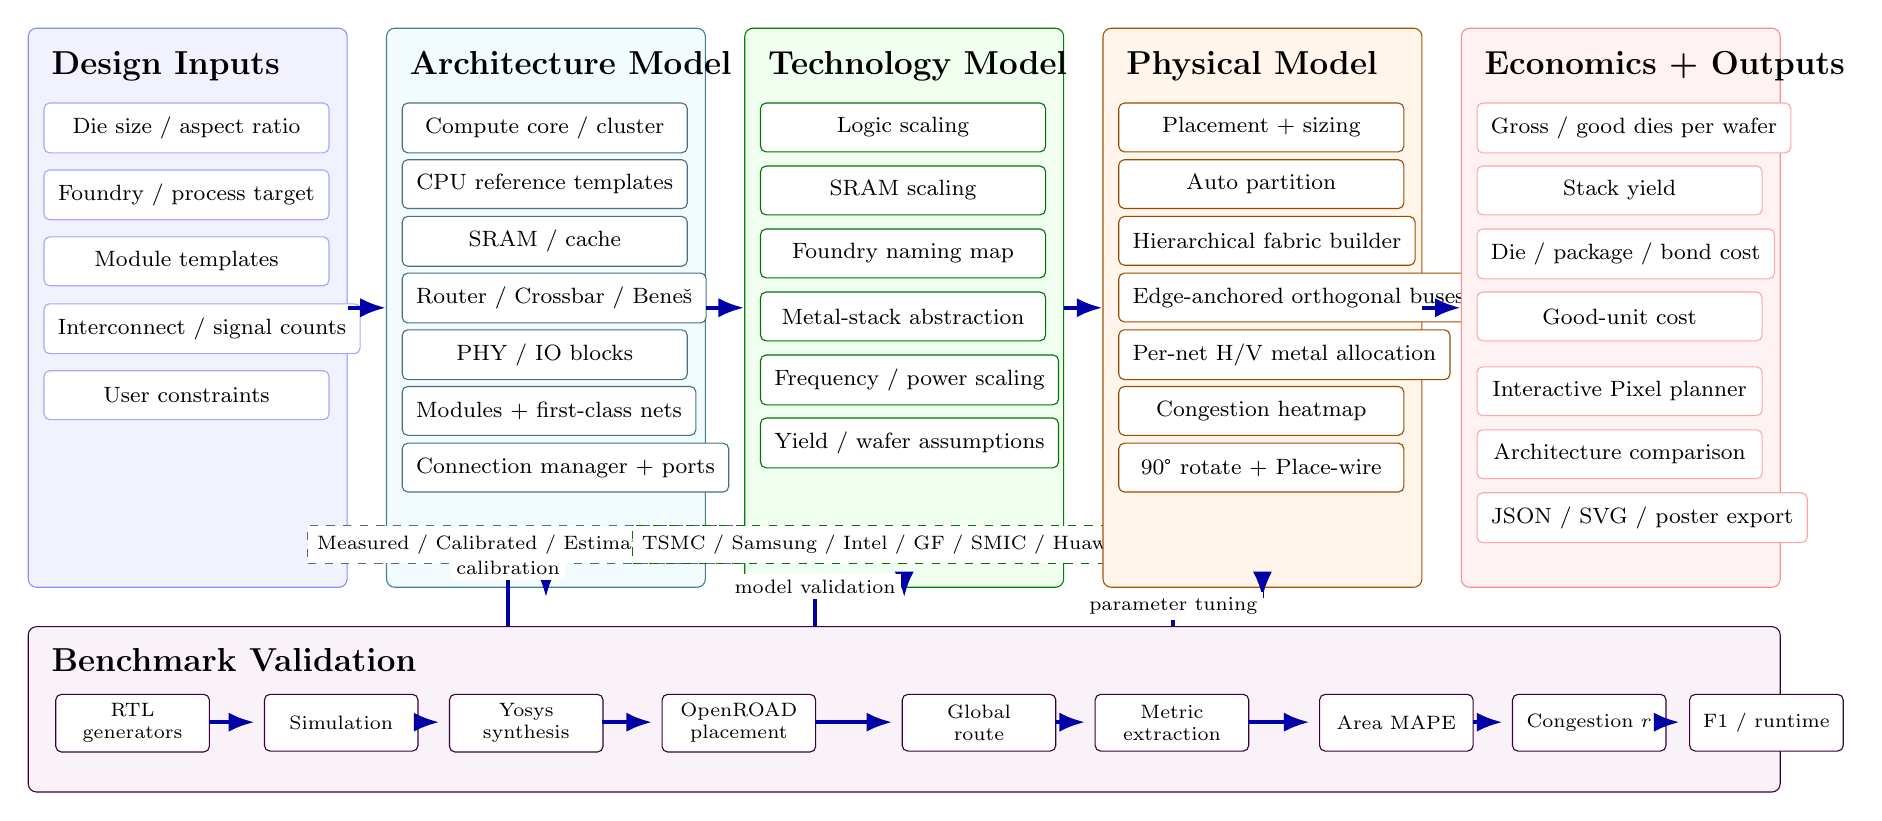
\begin{tikzpicture}[font=\sffamily,>=Latex,node distance=0pt]
\tikzset{col/.style={rounded corners=3pt,minimum width=4.05cm,minimum height=7.1cm,align=left,anchor=north west,inner sep=6pt}, item/.style={rounded corners=2pt,minimum width=3.62cm,minimum height=.62cm,align=left,anchor=north west,inner sep=5pt,font=\footnotesize}, title/.style={font=\bfseries\large,anchor=north west}, flow/.style={-Latex,line width=1.4pt,draw=blue!65!black}}
\node[col,fill=blue!5,draw=blue!45] (in) at (0,0) {};
\node[title] at ($(in.north west)+(0.18,-0.18)$) {Design Inputs};
\foreach \y/\t in {0.95/{Die size / aspect ratio},1.80/{Foundry / process target},2.65/{Module templates},3.50/{Interconnect / signal counts},4.35/{User constraints}}{\node[item,fill=white,draw=blue!35] at ($(in.north west)+(0.2,-\y)$) {\t};}
\node[col,fill=cyan!5,draw=cyan!55!black] (arch) at (4.55,0) {};
\node[title] at ($(arch.north west)+(0.18,-0.18)$) {Architecture Model};
\foreach \y/\t in {0.95/{Compute core / cluster},1.67/{CPU reference templates},2.39/{SRAM / cache},3.11/{Router / Crossbar / Bene\v{s}},3.83/{PHY / IO blocks},4.55/{Modules + first-class nets},5.27/{Connection manager + ports}}{\node[item,fill=white,draw=cyan!45!black] at ($(arch.north west)+(0.2,-\y)$) {\t};}
\node[font=\scriptsize,align=center,draw=cyan!45!black,dashed,fill=white] at ($(arch.south)+(0,0.55)$) {Measured / Calibrated / Estimated / Heuristic};
\node[col,fill=green!6,draw=green!50!black] (tech) at (9.10,0) {};
\node[title] at ($(tech.north west)+(0.18,-0.18)$) {Technology Model};
\foreach \y/\t in {0.95/{Logic scaling},1.75/{SRAM scaling},2.55/{Foundry naming map},3.35/{Metal-stack abstraction},4.15/{Frequency / power scaling},4.95/{Yield / wafer assumptions}}{\node[item,fill=white,draw=green!45!black] at ($(tech.north west)+(0.2,-\y)$) {\t};}
\node[font=\scriptsize,align=center,draw=green!45!black,dashed,fill=white] at ($(tech.south)+(0,0.55)$) {TSMC / Samsung / Intel / GF / SMIC / Huawei Tao};
\node[col,fill=orange!8,draw=orange!65!black] (phys) at (13.65,0) {};
\node[title] at ($(phys.north west)+(0.18,-0.18)$) {Physical Model};
\foreach \y/\t in {0.95/{Placement + sizing},1.67/{Auto partition},2.39/{Hierarchical fabric builder},3.11/{Edge-anchored orthogonal buses},3.83/{Per-net H/V metal allocation},4.55/{Congestion heatmap},5.27/{90\textdegree{} rotate + Place-wire}}{\node[item,fill=white,draw=orange!60!black] at ($(phys.north west)+(0.2,-\y)$) {\t};}
\node[col,fill=red!5,draw=red!45] (econ) at (18.20,0) {};
\node[title] at ($(econ.north west)+(0.18,-0.18)$) {Economics + Outputs};
\foreach \y/\t in {0.95/{Gross / good dies per wafer},1.75/{Stack yield},2.55/{Die / package / bond cost},3.35/{Good-unit cost},4.30/{Interactive Pixel planner},5.10/{Architecture comparison},5.90/{JSON / SVG / poster export}}{\node[item,fill=white,draw=red!35] at ($(econ.north west)+(0.2,-\y)$) {\t};}
% Main signals stay inside dedicated gutters.
\draw[flow] ($(in.east)+(0,0)$) -- ($(arch.west)+(0,0)$);
\draw[flow] ($(arch.east)+(0,0)$) -- ($(tech.west)+(0,0)$);
\draw[flow] ($(tech.east)+(0,0)$) -- ($(phys.west)+(0,0)$);
\draw[flow] ($(phys.east)+(0,0)$) -- ($(econ.west)+(0,0)$);
% Validation lane is separated below all main boxes.
\node[rounded corners=3pt,draw=violet!50!black,fill=violet!5,minimum width=22.25cm,minimum height=2.10cm,anchor=north west] (val) at (0,-7.60) {};
\node[font=\bfseries\large,anchor=north west] at ($(val.north west)+(0.18,-0.16)$) {Benchmark Validation};
\foreach \x/\t in {0.35/{RTL\\generators},3.00/{Simulation},5.35/{Yosys\\synthesis},8.05/{OpenROAD\\placement},11.10/{Global\\route},13.55/{Metric\\extraction},16.40/{Area MAPE},18.85/{Congestion $r$},21.10/{F1 / runtime}}{\node[rounded corners=2pt,draw=violet!45!black,fill=white,minimum width=1.95cm,minimum height=.72cm,align=center,font=\scriptsize,anchor=north west] at ($(val.north west)+(\x,-0.86)$) {\t};}
\foreach \a/\b in {2.30/2.88,4.95/5.23,7.30/7.93,10.00/10.98,13.05/13.43,15.50/16.28,18.35/18.73,20.80/20.98}{\draw[flow] ($(val.north west)+(\a,-1.22)$) -- ($(val.north west)+(\b,-1.22)$);}
% Feedback arrows use their own lane and label boxes.
\draw[flow] ($(val.north west)+(14.55,0)$) -- ++(0,0.38) -| ($(phys.south)+(0,-0.12)$);
\node[font=\scriptsize,fill=white,inner sep=2pt] at (14.55,-7.34) {parameter tuning};
\draw[flow] ($(val.north west)+(10.0,0)$) -- ++(0,0.62) -| ($(tech.south)+(0,-0.12)$);
\node[font=\scriptsize,fill=white,inner sep=2pt] at (10.0,-7.10) {model validation};
\draw[flow] ($(val.north west)+(6.1,0)$) -- ++(0,0.86) -| ($(arch.south)+(0,-0.12)$);
\node[font=\scriptsize,fill=white,inner sep=2pt] at (6.1,-6.86) {calibration};
\end{tikzpicture}}

\caption{Flash-flooplanner v8.6.1 methodology. Signal arrows occupy dedicated gutters between blocks; feedback arrows are routed below the main flow so that labels, boxes, and connectors do not overlap.}
\label{fig:framework}
\end{figure*}

\paragraph{Architecture model.}
The library contains generic logic, SRAM, compute cores and clusters, routers, crossbars, Bene\v{s} networks, arbiters, mux/demux blocks, PHYs, and CPU reference templates. CPU templates include Cortex-A55, Cortex-A76, Cortex-R82, BOOM configurations, XiangShan, Arm C1-Ultra, NVIDIA Vera Olympus, and Tenstorrent Ocelot. Tenstorrent Wormhole and Blackhole selectable templates are intentionally removed; Ocelot remains as the Tenstorrent CPU reference. Legacy projects that contain retired templates are preserved as fixed custom geometry rather than silently deleted.

\paragraph{Technology model.}
Logic and SRAM scale independently. Foundry-visible node names are mapped to internal model keys because commercial naming is not numerically interchangeable. SRAM capacity is converted using a node-dependent density and explicit macro overhead. Frequency and power scaling remain scenario assumptions, not guaranteed simultaneous PPA gains.

\paragraph{Physical model.}
Blocks have geometry, orientation, edge constraints, and routing blockage. Connections carry signal count, class, track factor, route preference, source/target edge anchors, and horizontal/vertical metal allocation. A coarse grid accumulates directional demand and compares it with available track capacity. Multi-tier W2W designs maintain separate tier yield and bonding yield terms.

\paragraph{Economic model.}
Gross dies per wafer, defect yield, bonding yield, package/test cost, and optional NRE amortization are kept distinct. For $N$ stacked tiers,
\begin{equation}
Y_{\mathrm{stack}}=\left(\prod_{i=1}^{N}Y_i\right)\left(\prod_{j=1}^{N-1}Y_{b,j}\right).
\end{equation}
When the yield denominator is zero the tool reports no good units instead of returning an artificially finite cost.

\paragraph{Evidence labels.}
Each major datum can be tagged Measured, Calibrated, Estimated, or Heuristic. The label is carried into reports so that a published architectural fact is not confused with a user-editable planning normalization.

\section{Connectivity and Editing Model}
A key v8.6.1 change is treating interconnect as a maintained list of design objects. A net records source and destination module IDs, physical signal count, track factor, traffic class, route mode, metal band, edge anchors, and the horizontal/vertical layer sets used by the bus. Hiding a net changes only visualization; it does not remove physical demand.

\subsection{Edge-Anchored Orthogonal Buses}
Each endpoint is represented as a module edge plus a normalized offset along that edge. Module translation therefore moves the endpoint without changing its semantic attachment. A $90^\circ$ rotation maps the edge and offset into the rotated coordinate system. The route generator exits and enters modules along edge normals and creates Manhattan segments between them. This removes the common visualization defect in which a thick connection appears to scrape along a module boundary rather than terminate on it.

The drawing separates a thin centerline, used for hit testing and route readability, from a translucent corridor representing estimated planar bus width. For a horizontal segment assigned a set $\mathcal{M}_H$ of legal layers, a first-order width estimate is
\begin{equation}
W_H \approx \frac{N_{\mathrm{track}}}{\sum_{m\in\mathcal{M}_H}\eta_m/p_m}+2g,
\end{equation}
where $p_m$ is routing pitch, $\eta_m$ is effective usable-track fraction, and $g$ is guard space. The vertical expression is analogous. Adding layers can reduce planar corridor width but does not reduce the number of physical signals. Shared layers remain shared resources; overlapping demands accumulate.

\subsection{Fast Editing}
The Place-wire mode, invoked by the toolbar or the \texttt{P} key, uses a two-click source/target interaction and previews the orthogonal route before committing it. The user can set signal count, net class, metal band, and H/V layer counts before placement. The Space key rotates a selected module clockwise by $90^\circ$; Shift+Space rotates counter-clockwise. Text-entry fields and IME composition suppress these shortcuts. Both operations enter the existing undo/redo history.

\subsection{Partition and Fabric Exploration}
The partition objective is
\begin{equation}
J=\alpha C_{\mathrm{cut}}+\beta C_{\mathrm{wire}}+\gamma C_{\mathrm{balance}}+\delta C_{\mathrm{congestion}}.
\end{equation}
The Architecture Lab compares a flat crossbar, hierarchical crossbar, Bene\v{s}, mesh, and ring using the same endpoint set and offered traffic. A candidate is applied only after explicit confirmation; previewing does not mutate the project. This comparison is heuristic and does not constitute a protocol, deadlock, or timing proof.

\section{Open-Source Benchmark Validation}
We use a deliberately narrow validation protocol so that measured evidence is not over-generalized. A fixed set of 18 RTL configurations spans parameterized crossbars, Bene\v{s} networks, and routers. The flow uses Icarus Verilog simulation, Yosys/ABC standard-cell mapping, and OpenROAD placement and global routing with the Nangate45 library. Each design is evaluated under nominal and constrained routing budgets where feasible.

Area calibration uses a small subset per family and evaluates held-out configurations. The target is mapped cell area, not final die area. Routing validation starts from an identical placed design and native OpenROAD GCell grid. The reference signal pressure subtracts resource-only usage from routed usage so that capacity reservations are not mistaken for signal demand.

Two prediction adapters are compared. The original v6 star adapter connects the source independently to sinks on the coarse grid. The experimental MST-plus-segment-union adapter builds a rectilinear approximation to shared trunks and avoids repeatedly charging identical segments of a multi-terminal net. Per-map Pearson and Spearman correlations measure spatial agreement. Hotspot F1 uses a threshold of directional demand/supply $\Gamma\ge0.8$ and is reported with a prevalence-aware all-positive baseline.

Runtime is separated into synthesis, placement, global route, and the planner-side prediction kernel. We do not divide millisecond kernel time by a complete RTL-to-route flow and call the ratio an end-to-end speedup, because the predictor in this experiment consumes placed pin locations.

\section{Results}
Table~\ref{tab:results} summarizes the held-out study. The calibrated structural area model achieves 24.87\% overall MAPE across 12 held-out designs. Family-level errors remain large enough that the model should be treated as an early budget, not a synthesis replacement.

\begin{table}[h]
\centering
\caption{Held-out validation summary.}
\label{tab:results}
\begin{tabular}{lrr}
\toprule
Metric & Original v6 & Improved adapter \\
\midrule
Area MAPE (12 tests) & \multicolumn{2}{c}{24.87\%} \\
Mean Pearson $r$ & 0.430 & 0.737 \\
Mean Spearman $\rho$ & 0.625 & 0.769 \\
Pooled hotspot F1 & 0.808 & 0.818 \\
Median predictor time & 3.01 ms & 9.35 ms \\
\bottomrule
\end{tabular}
\end{table}

The most important change is correlation, not F1. Under severely constrained routing, hotspot prevalence becomes so high that an all-positive classifier is competitive, making F1 alone misleading. The improved adapter better matches where demand concentrates while remaining several orders of magnitude lighter than a new physical-design run once placed geometry is available.

The benchmark also motivates current product behavior. Congestion is presented as a risk score with a Heuristic evidence label rather than a falsely precise signoff metric. Wide-net allocation across multiple H/V layers is accounted for as resource sharing rather than visual line thinning. Architecture comparisons expose wirelength, peak pressure, overflow cells, fabric area, estimated latency, and power side by side; the tool does not force the hierarchical candidate to win.

\section{Scope and Limitations}
The current model is intended for architecture-stage exploration. It does not perform detailed routing, extraction, static timing analysis, IR/EM analysis, thermal simulation, clock-tree synthesis, or signoff DRC. Process scaling from 28 nm toward advanced nodes is a calibrated abstraction assembled from public information and user-editable assumptions; it is not a substitute for a foundry PDK. Likewise, PHY depth, SRAM macro overhead, defect density, and wafer cost can dominate an actual product and must be replaced with project-specific data when available.

The Nangate45 experiment validates only the reported topology families, library, placement conditions, and congestion projection. Its correlations must not be transferred automatically to TSMC, Samsung, Intel, SMIC, GF, Huawei Tao, W2W stacks, or new CPU templates. CPU reference entries separate public architectural anchors from estimated physical budgets. Where cache or power data are uncertain, the UI exposes the assumption rather than presenting it as vendor measurement.

Future work should calibrate the connection model against multiple open PDKs, add obstacle-aware coarse routing, evaluate partition objectives using real netlists, and establish per-template synthesis baselines. A second direction is hierarchical multi-die exploration in which fabric, bonding-site, package escape, and thermal constraints are optimized jointly rather than independently.

\section*{Artifact}
Source and the interactive planner are available at \url{https://github.com/ldcyes/Flash-floorplan} and \url{https://ldcyes.github.io/Flash-floorplan/}. The planner is MIT licensed. This document is a preprint and is not an arXiv submission record.
\end{document}
